%%
%% This is file `sample-sigconf.tex',
%% generated with the docstrip utility.
%%
%% The original source files were:
%%
%% samples.dtx  (with options: `sigconf')
%% 
%% IMPORTANT NOTICE:
%% 
%% For the copyright see the source file.
%% 
%% Any modified versions of this file must be renamed
%% with new filenames distinct from sample-sigconf.tex.
%% 
%% For distribution of the original source see the terms
%% for copying and modification in the file samples.dtx.
%% 
%% This generated file may be distributed as long as the
%% original source files, as listed above, are part of the
%% same distribution. (The sources need not necessarily be
%% in the same archive or directory.)
%%
%% The first command in your LaTeX source must be the \documentclass command.
\documentclass[sigconf]{acmart}

% TODO remove XD
\usepackage{xcolor}
\newcommand{\secfunc}[1]{{\color{magenta}#1}}
\newcommand{\mention}[1]{{\color{cyan}#1}}
\newcommand{\plan}[1]{{\color{purple}#1}}
\newcommand{\bp}[1]{{\color{violet}#1}}
\newcommand{\draft}[1]{{\color{blue}#1}}
\newcommand{\review}[1]{{\color{black}#1}}
\newcommand{\todo}[1]{{\color{orange}(#1)}}

\usepackage{listings}

%%
%% \BibTeX command to typeset BibTeX logo in the docs
\AtBeginDocument{%
  \providecommand\BibTeX{{%
    \normalfont B\kern-0.5em{\scshape i\kern-0.25em b}\kern-0.8em\TeX}}}

%% Rights management information.  This information is sent to you
%% when you complete the rights form.  These commands have SAMPLE
%% values in them; it is your responsibility as an author to replace
%% the commands and values with those provided to you when you
%% complete the rights form.
\setcopyright{acmcopyright}
\copyrightyear{2020}
\acmYear{2020}
\acmDOI{10.1145/1122445.1122456}

%% These commands are for a PROCEEDINGS abstract or paper.
\acmConference[Seoul '20]{Seoul '20: Mining Software Repositories Data Showcase}{May 25--26, 2020}{Seoul, South Korea}
\acmBooktitle{Seoul '20: Mining Software Repositories Data Showcase,
  May 25--26, 2020, Seoul, South Korea}
\acmPrice{15.00}
\acmISBN{978-1-4503-9999-9/18/06}


%%
%% Submission ID.
%% Use this when submitting an article to a sponsored event. You'll
%% receive a unique submission ID from the organizers
%% of the event, and this ID should be used as the parameter to this command.
%%\acmSubmissionID{123-A56-BU3}

%%
%% The majority of ACM publications use numbered citations and
%% references.  The command \citestyle{authoryear} switches to the
%% "author year" style.
%%
%% If you are preparing content for an event
%% sponsored by ACM SIGGRAPH, you must use the "author year" style of
%% citations and references.
%% Uncommenting
%% the next command will enable that style.
%%\citestyle{acmauthoryear}

%%
%% end of the preamble, start of the body of the document source.
\begin{document}

%%
%% The "title" command has an optional parameter,
%% allowing the author to define a "short title" to be used in page headers.
\title{LogChunks: A Data Set for Build Log Analysis}

\author{Carolin Brandt}
\author{Annibale Panichella}
\author{Moritz Beller}

%%
%% By default, the full list of authors will be used in the page
%% headers. Often, this list is too long, and will overlap
%% other information printed in the page headers. This command allows
%% the author to define a more concise list
%% of authors' names for this purpose.
\renewcommand{\shortauthors}{Brandt, et al.}

%%
%% The abstract is a short summary of the work to be presented in the
%% article.
\begin{abstract}
Build failures are common in continuous integration (CI), but identifying the root cause of a failure is difficult.
Various tools have been proposed to boil down verbose build logs to the specific lines valuable to the developer.
We present \emph{LogChunks}, a collection of 797 Travis CI build logs from 80 GitHub repositories spread over 29 programming languages.
For each build log we manually labeled the log part (chunk) describing why the build failed.
We validated the data set by surveying the developers of the projects which produced the builds.
In addition, the data set categorizes the log chunks according to their format within the log text and provides keywords that a developer would use to search for the log chunks.
\emph{LogChunks} can be the basis to assess further build log analysis techniques and studies about why CI builds fail.


\end{abstract}

%%
%% The code below is generated by the tool at http://dl.acm.org/ccs.cfm.
%% Please copy and paste the code instead of the example below.
%%
%\begin{CCSXML}
%<ccs2012>
% <concept>
%  <concept_id>10010520.10010553.10010562</concept_id>
%  <concept_desc>Computer systems organization~Embedded systems</concept_desc>
%  <concept_significance>500</concept_significance>
% </concept>
% <concept>
%  <concept_id>10010520.10010575.10010755</concept_id>
%  <concept_desc>Computer systems organization~Redundancy</concept_desc>
%  <concept_significance>300</concept_significance>
% </concept>
% <concept>
%  <concept_id>10010520.10010553.10010554</concept_id>
%  <concept_desc>Computer systems organization~Robotics</concept_desc>
%  <concept_significance>100</concept_significance>
% </concept>
% <concept>
%  <concept_id>10003033.10003083.10003095</concept_id>
%  <concept_desc>Networks~Network reliability</concept_desc>
%  <concept_significance>100</concept_significance>
% </concept>
%</ccs2012>
%\end{CCSXML}
%
%\ccsdesc[500]{Computer systems organization~Embedded systems}
%\ccsdesc[300]{Computer systems organization~Redundancy}
%\ccsdesc{Computer systems organization~Robotics}
%\ccsdesc[100]{Networks~Network reliability}

%%
%% Keywords. The author(s) should pick words that accurately describe
%% the work being presented. Separate the keywords with commas.
\keywords{ci, build log analysis, build failure, chunk retrieval}

%%
%% This command processes the author and affiliation and title
%% information and builds the first part of the formatted document.
\maketitle

\section{Introduction}
Continuous Integration (CI) has become a common practice in software engineering~\cite{hilton2016usage}.
CI builds produce logs which report the progress and results of the steps within the build.
These build logs contain a lot of valuable information for developers and researchers.
Developers examine timer reports to track how different stages of the build process perform.
Researchers collect the commands triggering the build steps to reverse engineer the build configuration when only the log is available to them.
Both groups analyze build logs for descriptions of compiler errors, linter warnings or failed test notifications to uncover why a CI build failed~\cite{beller2017oops,seo2014programmers,vassallo2017a-tale}.

Build logs are verbose and long~\cite{beller2017oops}, making them inadequate for direct consumption.
Therefore, developers and researchers can only use the information within the build logs if they can adequately retrieve the parts (chunks) of the log that describe the targeted information.

There are different techniques to retrieve information chunks from CI build logs.
Beller et al.\ use regular expressions to analyze the reasons of build failures from Travis CI logs~\cite{beller2017oops}.
Such regular expressions are developed by looking at a few exemplary build logs. Updating them whenever new cases are introduced is a tedious and error-prone task~\cite{michael2019regexes}.
Vassallo et al.\ wrote a custom parser for build logs to gather information for build repair hints~\cite{vassallo2018un-break}.
Recently, Amar et al.\ reduced the number of build log lines for a developer to inspect by creating a diff between the logs from a failed and a successful build~\cite{amar2019mining}.

These approaches have various downsides and strengths:
Regular expressions are exact but difficult to maintain~\cite{michael2019regexes}.
Custom parsers are powerful though fragile towards changes in the log structure.
The structure of build logs changes from project to project~\cite{staahl2014modeling} as it depends on the tools and the environment used.
Taking a diff between failed and successful logs can reduce the information to be processed, but the imprecise output needs to be interpreted by a developer~\cite{amar2019mining}.
At the moment there is only anecdotal evidence on the performance of these techniques and when a technique should be preferred over other alternatives.
In addition, there is currently no data set available to evaluate and compare such chunk retrieval techniques for build logs.

We present \emph{LogChunks}, a collection of 797 Travis CI build logs from 80 GitHub repositories spread over 29 programming languages.
For each build log we manually labeled which substring describes why the build failed.
The data set also provides keywords a developer would use to search for the labeled log chunk and categorizes the log chunks according to their format within the log.

In this paper, we illustrate potential use cases of \emph{LogChunks} and present our own comparison of three chunk retrieval techniques using the data set.
Section \ref{sec:related-data-sets} describes related data sets and how \emph{LogChunks} differs from them.
The following section introduces the data schema, how to access the data set, as well as limitations and potential improvements.
We present our data collection in Section \ref{sec:data-collection}.
To validate our labels we performed a second labeling of a sample of the data.
In addition, we surveyed the developers, whose commits triggered the builds, whether our labeled log chunk describes why their build failed.
Section \ref{sec:validation} presents the two validation studies.
To conclude we describe limitations as well as potential improvements of \emph{LogChunks}.

We published \emph{LogChunks} through Zendoo: \todo{insert zendoo link}.

\section{Applications}
This section possible use cases for \emph{LogChunks} and outlines how we previously applied it to compare different build log analysis techniques.

\subsection{Potential Use Cases}
\emph{LogChunks} can be the basis for a wide range of further studies:

\paragraph{Evaluate Information (Chunk) Retrival Techniques}
In addition to the three techniques we investigated until now, \emph{LogChunks} can be the basis for evaluation and comparison of other chunk retrieval techniques.
We can use the data set to investigate how reliable the diff and information retrieval approach of Amar et al.~\cite{amar2019mining} retrieves the reason the build failed.

\paragraph{Support Build Log Classification Algorithms}
Various researchers are looking into why CI builds fail and use build logs as a data source~\cite{seo2014programmers,vassallo2017a-tale}.
They write custom parsers and classifiers to categorize builds according to why a build failed.
The manually labeled chunk describing why the build failed can show classification algorithms where in the build logs they can find the information relevant for the classification.

\paragraph{Analysis of Keywords Used to Search for Build Failure Descriptions}
\emph{LogChunks} provides keywords that a developer would look for to search the chunk describing why the build failed.
Analyzing these could help us understand how developers process build logs and which keywords a tool should use to mark an error description so developers quickly find it through text search.

\paragraph{Studying Conversations about Build Failures}
Some researchers are looking into conversations of developers surrounding CI builds and pull requests \todo{citation needed: nathan cassee did this in his master thesis (the paper on it is either rejected or not yet published), did not find others yet that do this}.
The chunks describing why a build failed, or the results of chunk retrieval techniques trained on them, can support these researchers to detect when a conversation participant is referring to the build failure described in the log.


\subsection{Chunk Retrieval Evaluation}
We created \emph{LogChunks} to evaluate and compare different chunk retrieval techniques for build logs.
The first technique is based on synthesizing programs from examples using the Microsoft PROSE library.
A user provides a small number of examples to describe which text part the program should extract.
PROSE then synthesizes a program of regular expressions that is consistent with these examples.
We compared this extraction technique to a text similarity approach, which selects the lines of a build log which are most similar to the ones in the given user examples.
Lastly, we investigated searching for keywords that are associated with the given user examples.

The log chunks in this data set provided the examples for these techniques, the keywords were used to configure the keyword search.
The structural categories enabled us to measure how structurally similar the examples have to be for a technique to be applicable.

Our results show that program synthesis is well suited to retrieve information chunks from build logs when the targeted information is always presented in a structurally identical way and the user requires a high confidence in the precision and recall of the output.
Using text similarity is advisable when precision is valued higher than recall and we recommend keyword search when recall is valued higher than precision.
We present more detailed results, background and our study design in \todo{ref (preprint or so?) of full journal paper (or thesis?)}.

\section{Related Data Sets}
\label{sec:related-data-sets}
This section presents existing data sets of CI build logs and why \emph{LogChunks} is unique among them.

\subsection{TravisTorrent}
The \emph{TravisTorrent} data set~\cite{beller2017travistorrent} collects a broad range of metadata about builds on Travis CI\@.
It combines data accessible through the public Travis CI API~\cite{travisci2019apidoc}, related data from GHTorrent~\cite{gousios2013ghtorrent}, the corresponding git repository and data obtained through analysis of the build logs.
The data obtained through build logs contains the names of failing test cases, similar to the reason the build failed in \emph{LogChunks}.
However, these values are obtained through a manually developed parser, which only supports specific Ruby test runners and Java Maven or JUnit logs.
\emph{LogChunks} provides manually labeled data points on the description of the build failure reason for a much wider selection of programming languages.

\subsection{Travis CI Build Log Data Set}
Loriot et al.~\cite{loriot2019dataset, loriot2019styler} collected a large amount of Travis CI build logs from 130 github repositories to analyze their use of the Checkstyle plugin.
They selected Maven repositories that included the Checkstyle plugin and also used Travis CI\@.
Their data set only provides the plain build logs, whereas \emph{LogChunks} additionally provides manually labeled data about the chunk describing why a build failed.

\section{Data Schema}
\label{sec:data-schema}

% \begin{figure}[tbp]
% 	\centering
% 	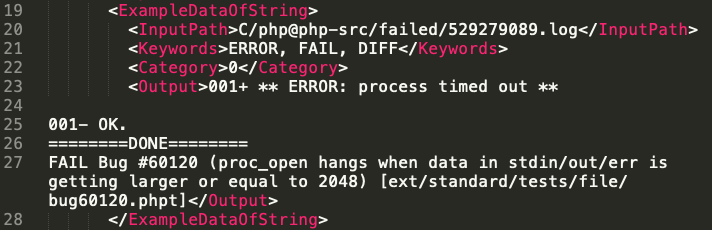
\includegraphics[width=0.45\textwidth, clip]{exampleXml.png}
% 	\caption{One example from the php/php-src repository in \emph{LogChunks}}
% 	\label{fig:dev-survey}
% \end{figure}

This section describes the file structure and the data schema of \emph{LogChunks}.
We give a detailed explanation for the manually labeled data.

\emph{LogChunks} has two top level folders, \texttt{logs} and \texttt{build-failure-reason}.
Each contains folders representing the main languages of the repositories in \emph{LogChunks}.

The logs are organized in folders for each repository, identified through the repository slug: \texttt{\textless repository\_owner\textgreater @\textless repository\_name\textgreater }.
Within each repository folder the logs are separated according to build status.
Currently \emph{LogChunks} only contains logs from \texttt{failed} builds.
The build status folder contains the full logs in files named with the ID of the Travis CI build that produced the log.

The folder \texttt{build-failure-reason} contains the manually labeled data of \emph{LogChunks}.
The data set provides an XML file for each repository \texttt{\textless repository\_owner\textgreater @\textless repository\_name\textgreater .xml}) categorized according to the main language of the repository.
The schema of these XML files is presented in Listing \ref{lst:examples}.

\lstset{
  language=XML,
  morekeywords={Examples, Example, Log, Keywords, Category, Chunk},
  postbreak=\mbox{\textcolor{blue}{$\hookrightarrow$}\space},
	frame=single
}
\begin{lstlisting}[caption={Example XML file from \emph{LogChunks}}, label=lst:examples, breaklines=true]
<Examples>
  <Log>C/php@php-src/failed/529279089.log</Log>
    <Keywords>ERROR, FAIL, DIFF</Keywords>
    <Category>0</Category>
    <Chunk>001+ ** ERROR: process timed out **

001- OK.
========DONE========
FAIL Bug #60120 (proc_open hangs when data in stdin/out/err is getting larger or equal to 2048) [ext/standard/tests/file/bug60120.phpt]</Chunk>
  </Example>
  ...
</Examples>
\end{lstlisting}

For each repository, \emph{LogChunks} gives about 10 \texttt{Examples}.
Each \texttt{Example} consists of:
\begin{itemize}
	\item \texttt{Log:} the relative path to the input build log.
	\item \texttt{Chunk:} the targeted information chunk. We are targeting the substring of the log that describes why the build failed.
	\item \texttt{Keywords:} keywords a developer would use to search for the log chunk.
	\item \texttt{Category:} a categorization of the structural representation of the log chunk within the build log.
				The category is relative to the other examples for the same repository.
\end{itemize}
Following, this section defines in more detail the labeled log chunk, search keywords and structural categories.

\paragraph{Chunk Describing Why The Build Failed}
The \texttt{Chunk} is the substring of the build logs that describes why the build failed.
This could be the failing test case, the description of a failed linter rule or a compiler error.
The \texttt{Chunk} is one continuous string cut from the build log.
If there are multiple errors leading for the build to fail, the substring contains the first appearing continuous error descriptions.
\emph{Continuous} means that no lines reporting of normal build behavior are interrupting the error descriptions.
Wherever possible, it does \emph{not} include the log statements describing \emph{that} the build failed, but the description of \emph{why} it failed.
For a few logs we were unable to define the section detailing why the build failed, e.g.\ because this information was logged in another log file.
In these instances the \texttt{Chunk} contains the lines describing that the build failed.

\paragraph{Keywords}
The \texttt{Keywords} contain a list of one to three keywords appearing within the \texttt{Chunk} or in the area around it in the build log.
We aim to select keywords a developer would use to search for the \texttt{Chunk} when inspecting the build log.

\paragraph{Category}
For each repository, we assign \emph{structural categories} to the examples.
The structural category compares how the \texttt{Chunk}s are represented within the build logs.
Build tools highlight their error messages with markings, e.g.\ starting each line with ``\texttt{ERROR}'', surrounding lines filled with special characters or additional empty log lines.
Two examples fall into the same structural categories if they are surrounded by similar markings.
For most cases, two \texttt{Chunk} examples that fall into one category are outputted either within the same build phase or by the same build tool.
For each repository, the structural categories are represented as integers, starting at 0 and increased with the next appearing category in chronological build order.

\section{Data Collection Process}
This section presents how we gathered the logs for \emph{LogChunks} and our manual labeling process.
\label{sec:data-collection}

\subsection{Log Collection}
We describe how we select the repositories, builds and logs for \emph{LogChunks}.
To collect the build logs we built the  \texttt{GHTorrentParser}, \texttt{LogCollector} and \texttt{TravisRequester} using Ruby.

\paragraph{Repository Sampling}
First, we determine a set of repositories to query logs from.
Our \texttt{GHTorrentParser} queries the \emph{GHTorrent}~\cite{gousios2013ghtorrent} data set for the most popular languages on GitHub~\cite{github2019website}.
It then retrieves the most popular repositories for a given language.
We define \emph{Popularity} as the number of watches.
The \texttt{TravisRequester}, our tool querying the Travis API~\cite{travisci2019apidoc}, can then check for a given repository whether it uses Travis CI\@.

For \emph{LogChunks} we queried GHTorrent from 01/04/2018 for the three most popular repositories of each of the 30 most popular languages.

\paragraph{Build Sampling}
The \texttt{LogCollector} uses the \texttt{TravisRequester} to obtain the newest builds for a given repository.
It uses a stratified sampling approach: \texttt{TravisRequester} saves the obtained builds in buckets according to their status.
We encountered the following statuses during our data collection: created, started, cancelled, passed, errored and failed.
The user of \texttt{TravisRequester} configures how many builds should be checked and how many builds per status should be saved.

To sample the builds for \emph{LogChunks} we let \texttt{TravisRequester} check up to a 1000 builds per repository and keep ten for each status.
We discard all statuses except \emph{failed}~\cite{travis2009buildstatus}.
A Travis CI build is marked as \emph{failed} when it faults in the \texttt{script} section of the build configuration defined by the user.

\paragraph{Log Sampling}
For each build the \texttt{TravisRequester} then selects a log to download.
Travis CI attributes logs to \emph{jobs}.
A single build can consist of multiple jobs, e.g.\ building the same code version and executing tests in various different testing environments.
A failed build can have successful job executions, as just one failed job leads to the whole build being marked as failed.
\texttt{TravisRequester} queries each build for the first job, which has the same state.
For the selected jobs, the tool queries the Travis API V3 over HTTPS to obtains the corresponding build log.

We manually inspected the collected build logs and had to discard logs from three repositories.
One had only a single failed build, two others had empty build logs on Travis CI\@.
In total we collected 797 logs from 80 repositories.

\subsection{Labeling Process}
\label{sec:labeling-process}
After collecting a wide range of Travis CI build logs we manually labeled which text chunk describes why the build failed.
Following that, we assigned search keywords and structural categories to each log chunk.

\paragraph{Chunk Describing Why The Build Failed}
For each repository, the labeler skimmed through the build logs and tried to identify the first occurrence of a description why the build failed.
They copied out the first continuous description as the \texttt{Chunk}.
They preserved whitespace and special characters, as they might be crucial to detect the targeted substring.
To support exact learning of regular expressions identifying the labeled substrings the labeler aimed to start and end the labeled substring at consistent locations around the fault description.

\paragraph{Keywords}
We presented the \texttt{Chunk} and ten lines above and below to the labeler.
Their task was to note down three strings they would put into a document search function to find this failure description.
The string should appear in or around the \texttt{Chunk} substring and is case-sensitive.
There are no special limitations on the string itself, especially spaces are also allowed.

\paragraph{Category}
To label the \emph{structural categories} we again presented the \texttt{Chunk} and the surrounding context to the labeler for all logs from a repository.
We asked them to assign numerical categories according to whether the \texttt{Chunk} had the same structural representation, i.e.\ the same surrounding or identifying characters.
The labeler should start the categories with 0 and increase as new ones appear.
For reproducibility we presented the logs in chronological build order.


\section{Data Set Validation}
\label{sec:validation}
We validate our collected data points in two different ways.
A different labeler performed a second pass of labeling the build failure reason, keywords and structural categories on a subset of the data.
In addition, we sent out a survey to the developers, whose commits triggered the builds within our data set.
We asked them whether our retrieval of the log part describing the reason the build failed was correct.
This sections describes these two validation studies.

\subsection{Inter-Rater Reliability Study}
To evaluate the validity of our labeled data points we perform a second labeling of a sample of the data in \emph{LogChunks}.

\paragraph{Method}
The second labeler processed 30 random generated logs for each data point in \emph{LogChunks}.
We followed the same labeling process as described in Section~\ref{sec:labeling-process}.
For the build failure reason and the keywords, we presented 30 randomly sampled build logs from distinct repositories in \emph{LogChunks}.
The labeled structural categories are relative to the other logs from the same repository.
Therefore, we randomly sampled 3 repositories and presented all 10 examples within them to the second labeler.

\paragraph{Results}
For the first labeled data point, namely the substring describing why the build failed, the two labelers exactly agreed in six cases.
In 15 cases the second labeler selected more lines than the first one, in five there was partial overlap and in 4 they completely disagreed.

Regarding the keywords the two labelers completely agreed in nine cases and completely disagreed in two cases.
In nine cases there was partial overlap in the keywords of the two labelers, in two the first labeler selected additional keywords compared to the second, while the second labeler proposed additional keywords in seven cases.

When classifying the labeled substrings into structural categories, the two labelers agreed in 26 cases and disagreed in four cases.

\paragraph{Discussion}
The results of this validation study show that there is overlap in the data from both labelers, however also a high variation.
We believe that the main cause for this is that our explanations to the second labeler were not extensive enough.
There were implicit, inconsistent assumptions both labelers created during their work.
In the following we describe these assumptions from both labelers for each data point and the implications on our description of the data classes.

For the first data class, the reason the build failed, it was ambiguous whether the labeled substring should contain the information \emph{that} the build failed.
This concerns statements like ``\texttt{The build exited with 1}''.
One labeler included such statements, while the other one only focussed on the log parts describing \emph{why} the build failed, e.g.\ the name of the failing test case.

While labeling the keywords a developer would use to search for the log part describing why the build failed, the one labeler allowed arbitrary strings appearing around the presented log part.
In contrast to that, the other labeler focussed on actual \emph{words}, delimited by spaces or special characters.
One labeler ignored capitalization, while the other one selected case-sensitive keywords.
A third difference was that the first labeler was presented with all substrings from a repository, yielding more general keywords than the second labeler.

For the structural categories this validation study showed a high overlap.
In our instructions to the second labeler we did not emphasize the \emph{structural} aspect enough.
They sorted into categories along \emph{why} the build failed, putting failing tests from different test runners into the same category even though the failing tests were presented differently in the log.

Our main learning from this study is that adequately communicating all decisions and assumptions on how data is labeled is important and difficult.
We reviewed the misunderstandings and incorporated more thorough descriptions of our data classes in Section~\ref{sec:data-schema}.


\subsection{Developer Survey}
For \emph{LogChunks} we analyzed around 800 build logs from different repositories and tried to extract the part of the log which describes why the respective build failed.
As we are not involved in the development of any of the projects within our data set we could only rely on our previous experience with various build logs and systems.
We only took the logs into accont and did not check the related configurations, so it is well possible that we extracted parts that do describe errors but the respective step failing is ignored by the configuration and the build failed for another reason.

The person who probably knows best why a build failed is the one committing the changes which triggered the build.
If the build was e.g.\ part of a pull request then developer likely inspected the failed build and tried to fix the build so the pull request can be accepted.
We sent out mails to the original developers whose commits triggered the builds represented in \emph{LogChunks} and asked them whether the log chunk we labeled actually describes why the build failed.
This section describes out survey and discusses our results.

\paragraph{Method}
Using the Travis API, for every build log in the data set we looked up the corresponding build and the committer information.
We grouped all commits triggered by one developer and sent out a mail to each of them, asking whether the log part selected during our labeling was indeed describing the reason the build failed.
%Figure~\ref{fig:dev-mail} shows one of the mails sent out.
The mail included links to the corresponding commits, build overview and log file.
We asked the receivers to fill out a short survey in case our extraction was not correct.
%Look at Figure~\ref{fig:dev-survey} to get an impression of the survey.
In the survey we presented the selected log part and asked the developer to paste in the log part actually describing the failure reason or describe why we were wrong in their own words.
As some of the extractions we labeled are many lines long, we trimmed all down to 10 lines to keep the mail readable.

\paragraph{Results}
In total we sent out mails to 246 developers, asking about 3.2 build logs per mail on average.
32 of these mails could not be delivered, e.g.\ because they were addressed to \emph{noreply} mail addresses.
These 32 mails related to 68 of the build logs.
We received answers from 61 developers, responding about 144 build logs.
%Figure~\ref{fig:mails-answers-received-mails} and Figure~\ref{fig:mails-answers-received-builds} show the proportions of mails and logs answered about, not delivered and unanswered.

Of the 144 answers, 132 said our extraction was correct.
26 answered either ``close, but not quite correct'' or ``no, the build failed for another reason''.
We manually inspected these negative answers and found that some extractions were correct after all.
This yields 12 log extractions in our example set that were not correct.%, shown in Figure~\ref{fig:mails-extraction-correct}.

\paragraph{Discussion}
This study highly strengthens the trust in the validity of the extracted build failure reasons in \emph{LogChunks}.
The study received answers about 18\% of the logs from \emph{LogChunks}.
After manual correction, 91\% of the received answers said our labelled extractions were accurate.

Most of the initial incorrect answers we adjusted in the manual correction, stated that the proposed extraction did not show the whole description of why the build failed.
This is because we had to trim long labeled extractions to keep the mails readable.

One of our extractions only showed a warning and the developer proposed to also include the line above, stating that warnings are treated as errors in the build.
In others that were identified as incorrect, we labelled the error message of an error that later ignored and did not lead to the build failing.

\section{Conclusion}
In this paper we introduced the \emph{LogChunks} data set encompassing about 800 build logs from a wide range of projects using Travis CI.
For each log we annotated the log chunk describing why the build failed and provide keywords a developer would use to search for the log chunk as well as a categorization of the log chunks according to their format within the log.
Still there are limitations to our data set, which we present in the following.
We also propose several improvements and extensions to \emph{LogChunks}.
\label{sec:conclusion}

\paragraph{Chunk as One Consecutive Substring}
The manually labeled \texttt{Chunk} in our data set aims to contain the log part describing why the build failed.
However, it contains only one consecutive substring of the log text, whereas the reason a build failed could be described at multiple locations within the log.
We could improve this by extending \emph{LogChunks} to contain multiple substrings of the log text.

\paragraph{Include More Repositories and Logs}
\emph{LogChunks} encompasses a wide range of repositories from various main development languages, though only 10 logs from each repository.
This stems from the high effort necessary for the manual data labeling process.
Including more logs and repositories into \emph{LogChunks} will strengthen it as a broad baseline for comparing build log analysis tools.

\paragraph{Classification of the Build Failure Cause}
Our data set contains the log chunks describing why a build failed but has no further classification according to the cause of the failure.
As various researchers are investigating why CI builds fail, a useful extension would be to annotate cause of the build failure for each log.

\paragraph{Other Targeted Information Chunks}
Build log analysis is not limited to retrieving the chunk describing why a build failed.
\emph{LogChunks} could be extended with further information targets such as descriptions of warnings, build infrastructure and more.

%%
%% The acknowledgments section is defined using the "acks" environment
%% (and NOT an unnumbered section). This ensures the proper
%% identification of the section in the article metadata, and the
%% consistent spelling of the heading.

% \begin{acks}
% To Robert, for the bagels and explaining CMYK and color spaces.
% \end{acks}

%%
%% The next two lines define the bibliography style to be used, and
%% the bibliography file.
\bibliographystyle{ACM-Reference-Format}
\bibliography{paper}

%%
%% If your work has an appendix, this is the place to put it.
% \appendix

% \section{Research Methods}

% \subsection{Part One}


\end{document}
\endinput
%%
%% End of file `sample-sigconf.tex'.
